\documentclass[letterpaper,12pt,notitle]{memphisthesis}                     % the template uses 12pt Arial, I use 12pt Times New Roman
\usepackage[lmargin=1in,rmargin=1in,tmargin=1in,bmargin=1in]{geometry}  % left margin of the original template has been modified
\usepackage[section]{placeins}  % noted by Yu Geng: use this opition to enforce figures to stay in the current section
% \usepackage[demo]{graphicx}   % noted by Yu Geng: use this to speed up compilation, comment it before final render

\usepackage{natbib}         % bibliography showing “and” instead of “&”
\newcommand\harvardand{\&}  % required by the University of Memphis Thesis Style Guide

%\usepackage{chngcntr}
%\counterwithout{figure}{chapter}  % consecutive numbering of tables and figures throughout the document
%\counterwithout{table}{chapter}   % required by the University of Memphis Thesis Style Guide

\usepackage{titlesec}               % move section and subsection titles to the left side a little bit
\titlelabel{\llap{\thetitle\quad}}  % suggested by the Graduation Analyst
\renewcommand\thesection{}     % remove numbering before any section, subsection... names
\renewcommand\thesubsection{}  % required by the University of Memphis Thesis Style Guide

%\usepackage[finalnew]{trackchanges}  % Accept all edits.
\usepackage[inline]{trackchanges}  % Display edits inline.
\addeditor{HC}  % arranged in alphabetical order
\addeditor{EC}  % arranged in alphabetical order


% noted by Yu Geng: usage of [] after \subfigure
% without using [], numbering of subfigures (a) and (b) will not show up
% contents in the [] can be just left as blank
% EXAMPLE
% \begin{figure}
%     \subfigure[]{...}
%     \subfigure[]{...}
%     ...
% \end{figure}

% If you want the fonts to be Times New Roman uncomment the following line 
\usepackage{times}

%If you want the fonts to be Times New Roman, comment out the following 3 lines
% \usepackage[T1]{fontenc}
% \usepackage[scaled]{uarial}
% \renewcommand*\familydefault{\sfdefault}

\usepackage{amsmath}
\usepackage{textcomp}
\usepackage{booktabs}
\usepackage{setspace}
\usepackage{graphicx}
\usepackage{subfigure}
\usepackage[justification=raggedright,
singlelinecheck=false]{caption}
\usepackage{indentfirst}
\usepackage[splitrule]{footmisc}

\setlength{\footnotemargin}{0.5in}
\setlength{\footskip}{0.5in} 

\makeatletter
\let\splitfootnoterule=\pagefootnoterule
\makeatother

\setcounter{tocdepth}{3}
\raggedright

\makeatletter
\let\l@figureOLD \l@figure
\renewcommand{\l@figure}{\vspace{\baselineskip}\l@figureOLD}
\let\l@tableOLD \l@table
\renewcommand{\l@table}{\vspace{\baselineskip}\l@tableOLD}
\makeatother

\setlength{\parindent}{0.5in}

\begin{document}

\pagenumbering{roman}

\begin{titlepage}

\vspace*{.66in}
\begin{center}\uppercase{
New Numerical Mid-Ocean Ridge Models for Interactions between plate-driving and resistant forces 
}\vspace{2em}\\  % \vspace{.34in}\\
by\\
\vspace{2em}  % \vspace{.34in}
Hee Choi
% Interactions between plate-boundary forces and evolving resistance at mid-ocean ridges as the origin of non-uniform seafloor growth

\vspace{1.5in}
A Thesis \\
\vspace{14pt}
Submitted in Partial Fulfillment of the\\ \vspace{14pt}
Requirements for the Degree of\\ \vspace{14pt}
Master of Science
\vspace{0.5in}

Major: Earth Sciences

\vspace{1.66in}
The University of Memphis \\
\vspace{14pt}
May 2019
\end{center}

\end{titlepage} 


\doublespacing
\widowpenalty=10000

\setcounter{page}{2}

\begin{center}
	\textbf{ACKNOWLEDGEMENTS}
\end{center}
\vspace{-0.15in}

Acknowledments~~

\newpage
\begin{center}
	\textbf{ABSTRACT}
\end{center}
\vspace{-0.15in}

\thispagestyle{plain}

\note[Geng]{Abstract shortened according to University of Memphis Thesis Style Guide.} Abstract will be here.

\newpage

\begin{singlespace}
	\tableofcontents
\end{singlespace}

\newpage

\addcontentsline{toc}{chapter}{List of Figures}

\addtocontents{lof}{\vspace*{-\baselineskip}}

\begin{singlespace}
	\listoffigures
\end{singlespace}

\newpage

\pagenumbering{arabic}

\chapter{Introduction}
\setcounter{section}{0}
\setcounter{subsection}{0}

Mid-ocean ridge systems have been extensively studied because of their unique geological and geophysical characteristics as well as their importance in global plate tectonics. Being the longest mountain belt on the Earth, mid-ocean ridges have a total length of 80,000 km and cover over 23 percent of the Earth’s surface \citep{Peltier1989}. Stripe patterns of magnetic anomalies parallel to the mid-ocean ridge are critical evidence for seafloor spreading and the birth of plate tectonics \citep{Hess1964}.

The mid-ocean ridge is the place where new oceanic crust and lithosphere are generated by partial melting of the upper mantle \citep{Cann1968}. Magma rising from the upper mantle extrudes onto the ocean floor and bonds to the edges of separating plates \citep{Chen1992}. The oceanic plates start thin and thicken by the underplating of new lithosphere from the upper mantle and the accumulation of overlying sediment layers. As it moves away from the ridge, the lithosphere is getting cooler and denser.

%\note[EC]{You need to mention Chen and Morgan JGR 199X. Refer to Fowler's Solid Earth book's chapter on mid-ocean ridge.} \note[HC]{Do you mean I should wirte a paragraph talking about thermal/rheology models of MOR?} \note[EC]{Yes. In addition, this is the place where you should boast of your knowledge on the topic. Summarize all the relevant work on mid-ocean ridge: e.g., other works by Reston, Ranero, Cannat, Canales, Escartin, Buck, Tucholke, Ito, Behn, Olive, Tian and Choi. It doesn't have to be an encyclopedic article but a thesis's introduction should be sufficiently comprehensive.}

Previous studies for mid-ocean ridges have improved our understanding about how rheological and thermal structure affect the faulting at the mid-ocean ridge system.
%\citet{Lavier2002} suggested that the hydrothermal circulation determine the style of faulting on both half grabens and large-offset low-angle normal fault.\note[EC]{Lavier2002 seems out of context. Maybe later when you discuss large-offset normal fault?} 
\citet{Chen1990} coupled the thermal and rheologic field in a model of lithospheric stretching to consider the controls on axial relief at mid-ocean ridges. The spreading rate dependence of axial valley morphology is well predicted by including a weak lower crust. \citet{Behn2008} suggested that a number of factors including lithospheric structure and rheology controls fault growth, although the dominant factor is the ratio of magmatic accretion to the rate far field extension. \citet{Singh2006} provided first seismic reflection image of subsurface near-magma chamber at slow-spreading ridges and a series of inward-dipping faults cutting through the volcanic edifice, suggesting continuous interplay between magmatic and tectonic processes. \citet{Olive2015} looked at the patter of faulting by varying the period of magmatic fluctuation. Increasing the period of fluctuating magma supply in the model generates long-wavelength topography with large-offset faults.

Numerical models including relationship between dike opening rate and plate separation have also contributed to the knowledge of mid-ocean ridge.
\citet{Buck1998} developed a simple way to parameterize the complex process of magmatic accretion at a spreading center. This numerical model assumes steady accretion of crust at the spreading center. \citet{Buck2005} and \citet{Tucholke2008} showed that differences in magmatic input to dikes produce the different modes of faulting at mid-ocean ridges. When magmatic accretion accommodates 30-50\% of spreading, the model generates detachment faults while the model shows alternating faulting mode when most of spreading is accommodated by magmatic accretion. \citet{Tian2017} used three-dimensional model to quantify the effects of axially variable diking rates on faulting at slow spreading ridge segment and newly identified transitional mode. Varying the amount of magma supply along the spreading axis result in two different faulting modes in one model.

\note[HC] {IDK how I can group this sentence with others, suggestions?}
\citet{Reston2011} claimed that both a large-offset normal fault and a series of comparatively small fault blocks are likely to originate through a rolling hinge mechanism, caused by the flexure of the footwall during unloading. When the fault locks up at adequately high angle, a new fault propagates upwards from the active root zone. Repeating these process produces a series of small rafting fault blocks.

\begin{figure}[!htb]
	\centering
	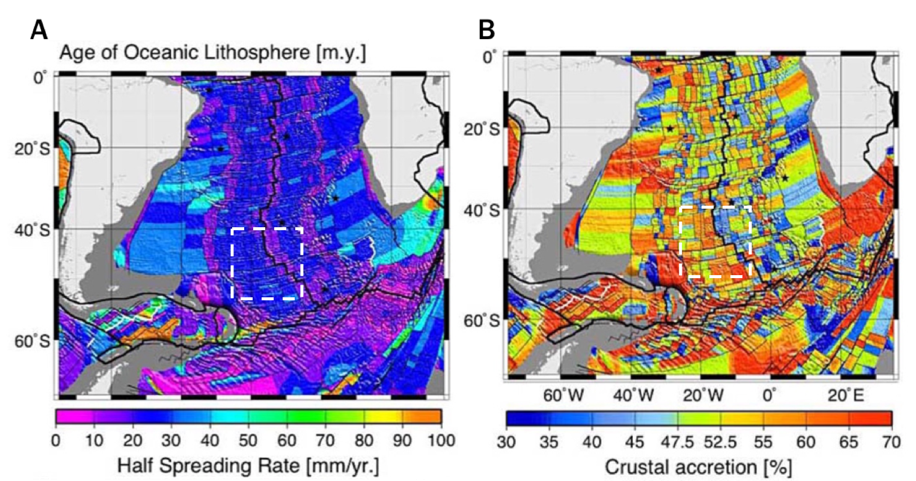
\includegraphics[width=0.9\linewidth]{./figs/hsr_muller.png}
	\caption{\textbf{A.} Seafloor half-spreading rates. \textbf{B.} Crustal accretion asymmetries in the South Atlantic, Scotia Sea, and northern Weddell Sea. Dashed boxes in A and B mark the region clearly showing asymmetric features. Modified from \citet{Muller2008}}
	\label{fig:hsr_muller}
\end{figure}

These previous studies have assumed the accretion of oceanic lithosphere at spreading centers to occur symmetrically and at a constant rate, but this assumption is not consistent with various observations \citep{Castelino2016, Flament2014, Martinez2006, Muller1998, Muller2008, Fedotova2017}. \citet{Castelino2016} explained anomalous bathymetry of the Mozambique basin and Riiser Larsen sea with the presence of thicker-than-usual oceanic crust older than 100 Ma. \citet{Flament2014} suggested that viscous lower mantle flow may represent topographic asymmetry of the South Atlantic. \citet{Martinez2006} identified non-corresponding trends in crustal thickness and spreading rate along the back-arc Eastern Lau Spreading Center. \citet{Muller2008} set the new set of digital grids computing global depth anomalies, showed age, spreading rates, and spreading asymmetry of the world’s ocean crust (Figure \ref{fig:hsr_muller}). The asymmetric plate growth is not only a specific regional observation, it is a worldwide feature.

\begin{figure}[!htb]
	\centering
	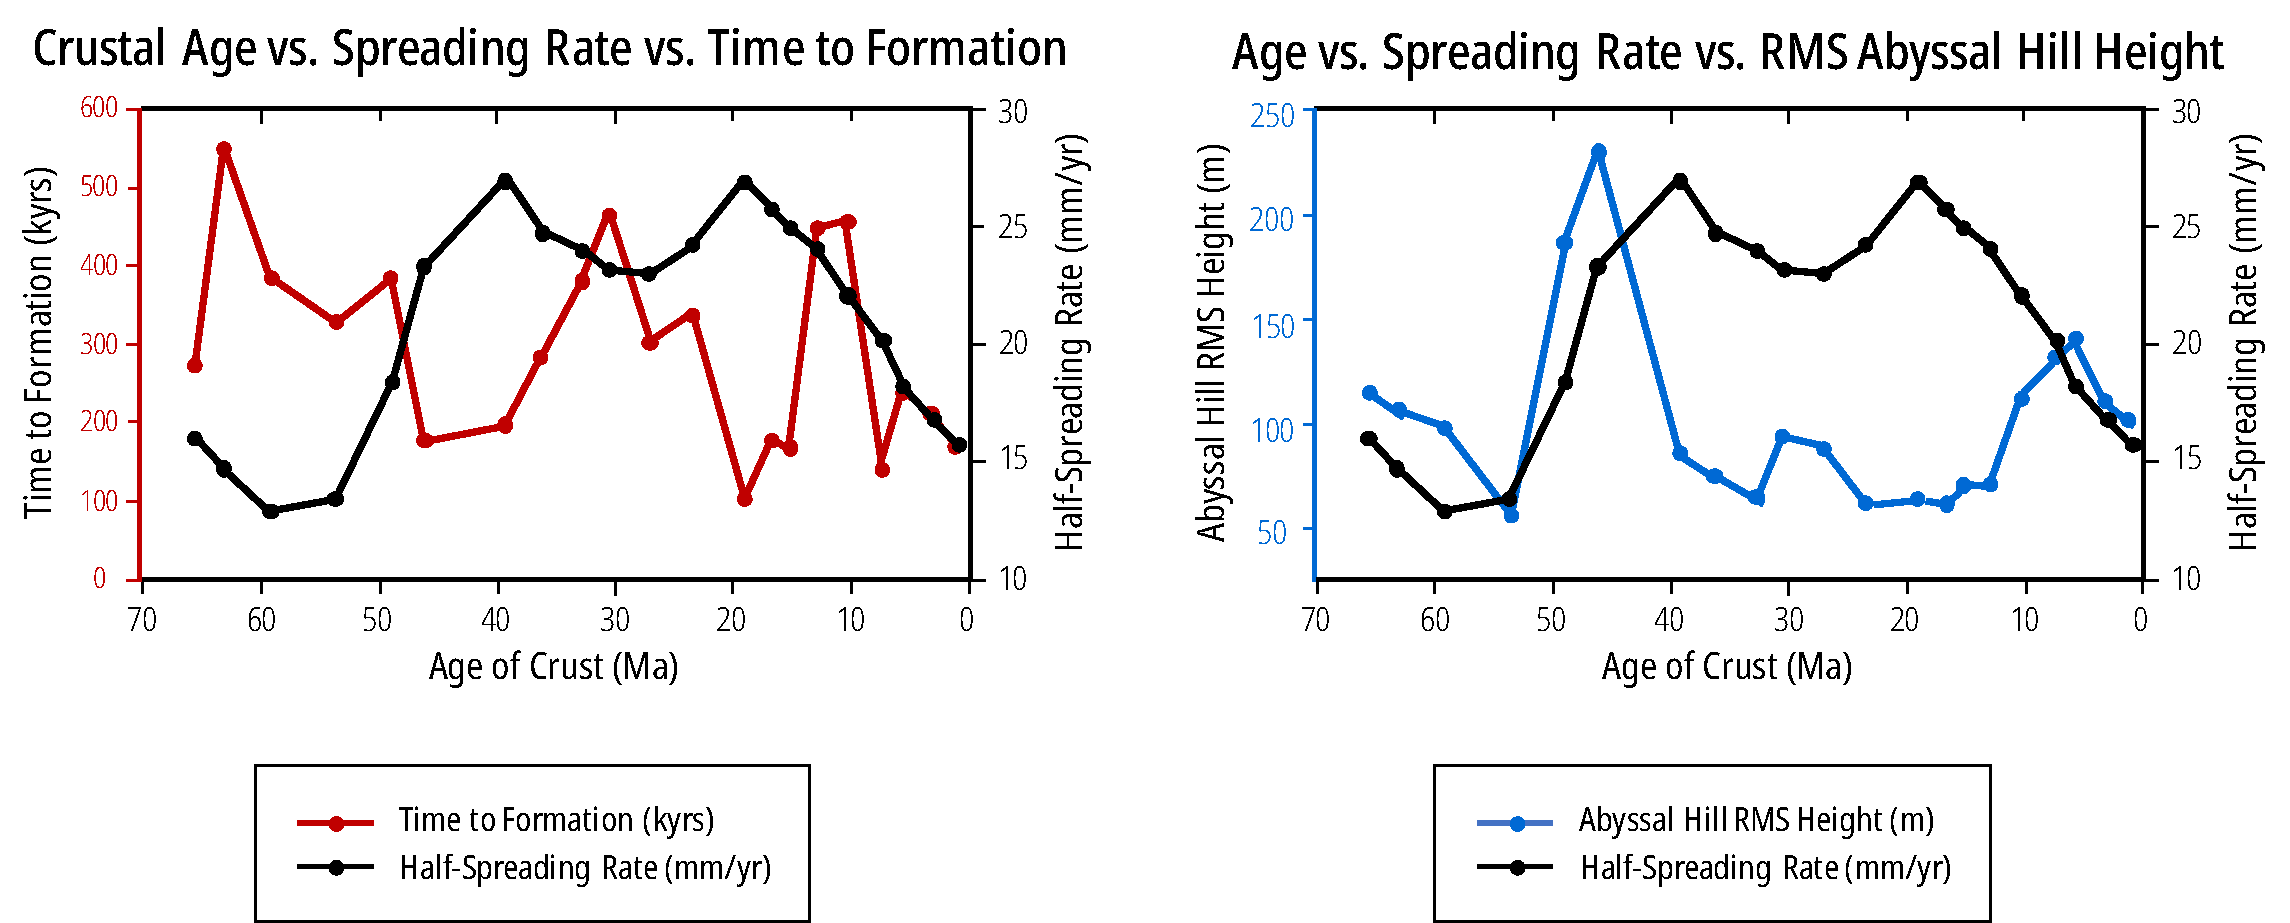
\includegraphics[width=0.99\linewidth]{./figs/hsrgraph1.pdf}
	\caption{Non-uniform half-spreading rate, abyssal height and time to form abyssal hill data from CREST expedition in mid-Atlantinc Ridge. Digitized from \citet{Fedotova2017}}
	\label{fig:hsr_fedotova}
\end{figure}

Recently from CREST expedition, \citet{Fedotova2017} observed the half-spreading rate, time to form abyssal hills and abyssal hill height vary on time  (Figure \ref{fig:hsr_fedotova}). %\note[EC]{Either combine these two figures into one or discuss them separately in separate paragraphs. Also, don't just throw figures in and leave readers unguided. The purpose and contents of a figure should be stated.} 
If plate grows at a constant rate, spreading rate and required time to form abyssal hill as time goes on will be a constant as well. Abyssal hill height will be plotted as a sinusoidal curve with regular amplitude and frequency by assuming uniform plate spreading. These observed data indicate that not only asymmetric between left and right plates from spreading center but also non-uniform plate growing behavior is observed on the seafloor.

Continental rifts, another type of divergent plate boundary, has recently been shown to form slowly during the incipient stage and accelerate later \citep{Brune2016}. Based on the kinematic modeling based on plate motion inversion data from the major passive margins North Atlantic, North America – Greenland, Australia – Antarctica, and the South China sea, \citet{Brune2016} identified several rapid changes in absolute plate motion from the extension records in the major passive margins around the world, which have not been explained previously. They explained the multi-phase rifting as a result of the interaction between the evolving strength of a rift zone and forces pulling the plates apart. At the initial stage of rifting, the lithosphere is still thick and strong and thus high strength let rifting slow (Figure \ref{fig:brune}A). When the lithosphere gets significantly thinned and weakened, low strength enables fast rifting (Figure \ref{fig:brune}B).

\begin{figure}[!htb]
	\centering
	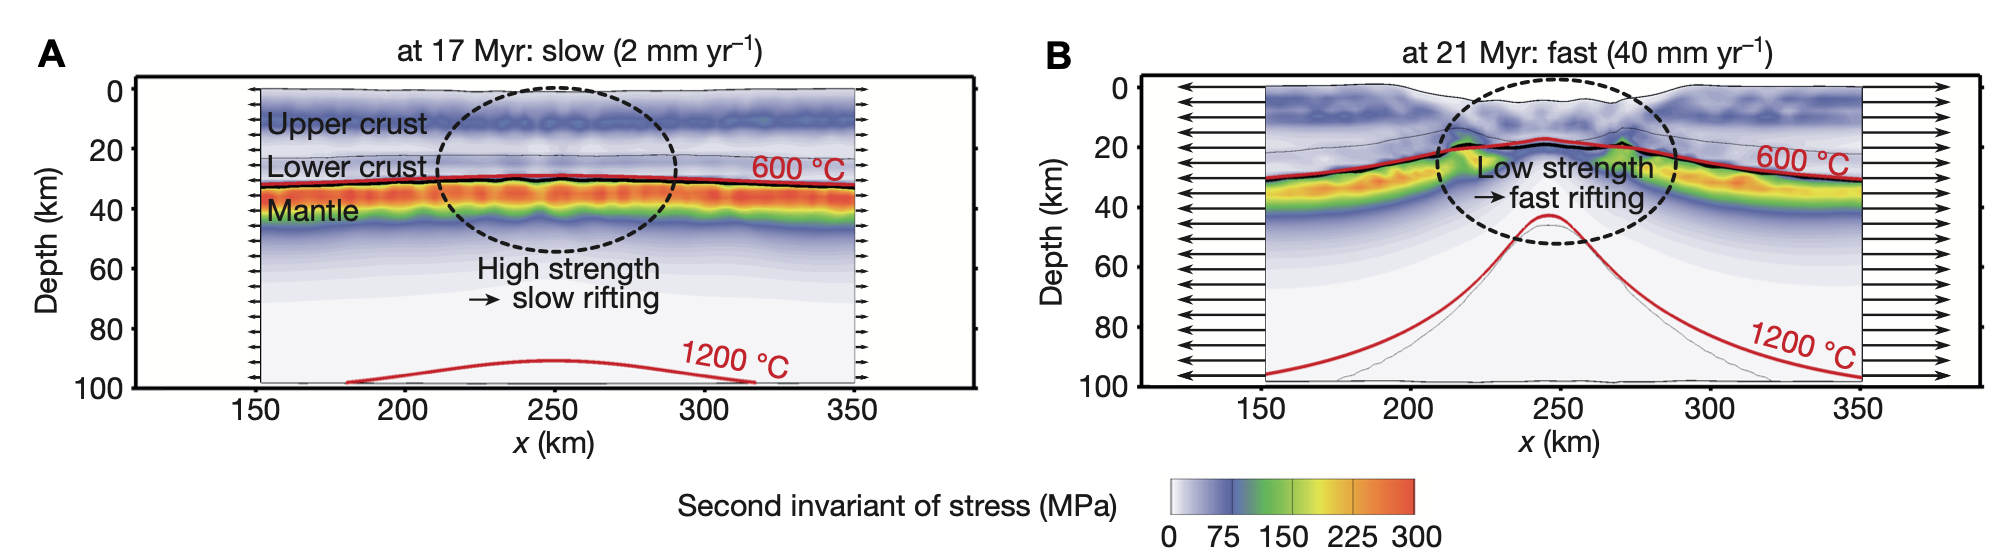
\includegraphics[width=0.99\linewidth]{./figs/brune.png}
	\caption{Strength evolution in numerical models for continental rifting with constant force boundary conditions. \textbf{A.} Distribution of the second invariant of stress at 17Myr when the lithosphere is still thick and strong and thus the extension rate is low, 2mm/yr. Arrows indicate extension velocity. \textbf{B.} After 21Myr when the lithosphere gets significantly thinned and weakened, letting the extension rate increase to 40 mm/yr. From \citet{Brune2016}}
	\label{fig:brune}
\end{figure}

Prompted by the non-uniform plate growth at mid-ocean ridges and potential interactions between the far-field forces and mid-ocean ridge processes, I investigate the mechanism of interactions between plate driving forces and internal forces at mid-ocean ridges including diking and faulting using numerical models. Conventional kinematic boundary conditions are replaced with tractions in numerical models for mid-ocean ridges. I also include magmatic intrusion and faulting at a spreading center in models because magmatism and faulting play a vital role in determining characteristics of mid-ocean ridges. 

\chapter{Modeling Method}

Magmatism at the spreading center of mid-ocean ridges plays an essential role in determining faulting styles that in turn control the axial and seafloor morphology. At fast-spreading ridges, copious magma rises and forms axial high (Figure \ref{fig:ridgebathymetry}A). With abundant magma, diking can occur frequently accommodating a significant portion of plate separation. For this reason, faults forming near axial highs have only small (i.e., 100s m) offsets (Figure \ref{fig:ridgebathymetry}A). Density variations are significant across fast-spreading ridges since the axial lithosphere is very thin, hot, and underlain by partially molten crust. Axial highs might originate from fluid magma rising to the level of local isostatic equilibrium at the plate spreading axis and then subsiding as it cools down. In contrast, faults forming at slow-spreading centers show greater offset, and axial valleys form at the spreading center (Figure \ref{fig:ridgebathymetry}B). Less abundant magma compared to fast-spreading ridges means less frequent diking and tectonic stretching accommodates a significant portion of plate separation. Faults at slow-spreading ridges develop offset up to 1-2 km. Abyssal hills produced at slow-spreading ridges are composed of faults dipping towards the axis while about half of the faults near fast-spreading centers dip toward the axis and the other half dip away from ridge axis.

\begin{figure}[!htb]
	\centering
	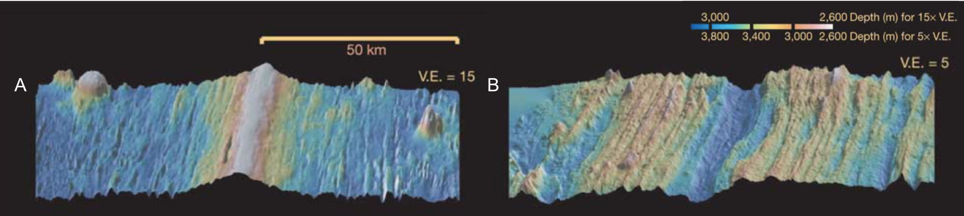
\includegraphics[width=0.99\linewidth]{./figs/bathy_buck.png}
	\caption{Shaded relief images of bathymetry at slow and fast ridges. \textbf{A.} The East Pacific Rise along 9$^\circ$37$'$N latitude \textbf{B.} The Southeast Indian Ridge along the 115$^\circ$E segment. Modified from \citet{Buck2005}.}
	\label{fig:ridgebathymetry}
\end{figure}

\citet{Buck1998} developed a simple way %\annote[EC]{simple way}{Explain what it is. Also, include a formal defintioni of their parameterization somewhere. If you do that, the description of Buck et. al (2005) would have to be in another paragraph.} 
that the presence of a magma-filled dike is assumed to enable shear displacement at negligible levels of shear stress. It parameterized the magmatic accretion at a spreading center as an amount of extension affected by steady intrusion of dikes. This approach allowed the lateral position of a modeled dike to explain the contrasting faulting styles at slow- and fast-spreading ridges.

In the \citet{Buck2005}'s model, dike openings in the lithosphere are taken to be uniform with depth and quantified by the ratio of dike opening rate to total plate spreading rate. This ratio is denoted as M and typically given as a parameter for a model so that the rate of diking-accommodated plate separation is determined as M times total spreading rate. When M = 0, dikes account for none of the plate spreading; and dikes accommodate all the plate separations when M = 1. M less than one corresponds to the case where magma supply is insufficient for filling the entire opening created by plate separation and tectonic stretching of the lithosphere should occurs. For M = 1, axial lithospheric separation is all taken up by dike widening and no faults and no axial valley develop.  For 0.5 $<$ M $<$ 1, faults develop and slip at a horizontal rate of (1$-$M) Vp (Figure \ref{fig:mfactor}A). Since the opening by diking is faster than the rate that the fault offset increases, the fault itself is pushed off axis with time. When pushed far away from the axis, the fault locks because the lithosphere around the fault becomes thicker and stronger. As a result, a new fault forms at the spreading center, continuing to accommodate a part of plate separation. For M = 0, dikes account for none of the plate spreading. Results for stretching-dominated ridge models are illustrated in Figure \ref{fig:mfactor}B and C. In the case of M = $\sim$1, the model produces a symmetric pattern of small-offset faults, producing a bathymetric profile similar to that of the Southeast Indian Ridge (Figure \ref{fig:mfactor}B). For M = 0.5, the model generates two large offset faults on one side, and a series of small faults on the other side. Lithospheric stretching creates conjugate normal faults at the spreading center initially. Only one branch survives on one side of the ridge, eventually evolving into a detachment fault, while short-lived new faults semi-regularly form on the opposite side. The resultant bathymetric profile resembles that of the slow-spreading Mid-Atlantic Ridge (Figure \ref{fig:mfactor}C).

\begin{figure}[!htb]
	\centering
	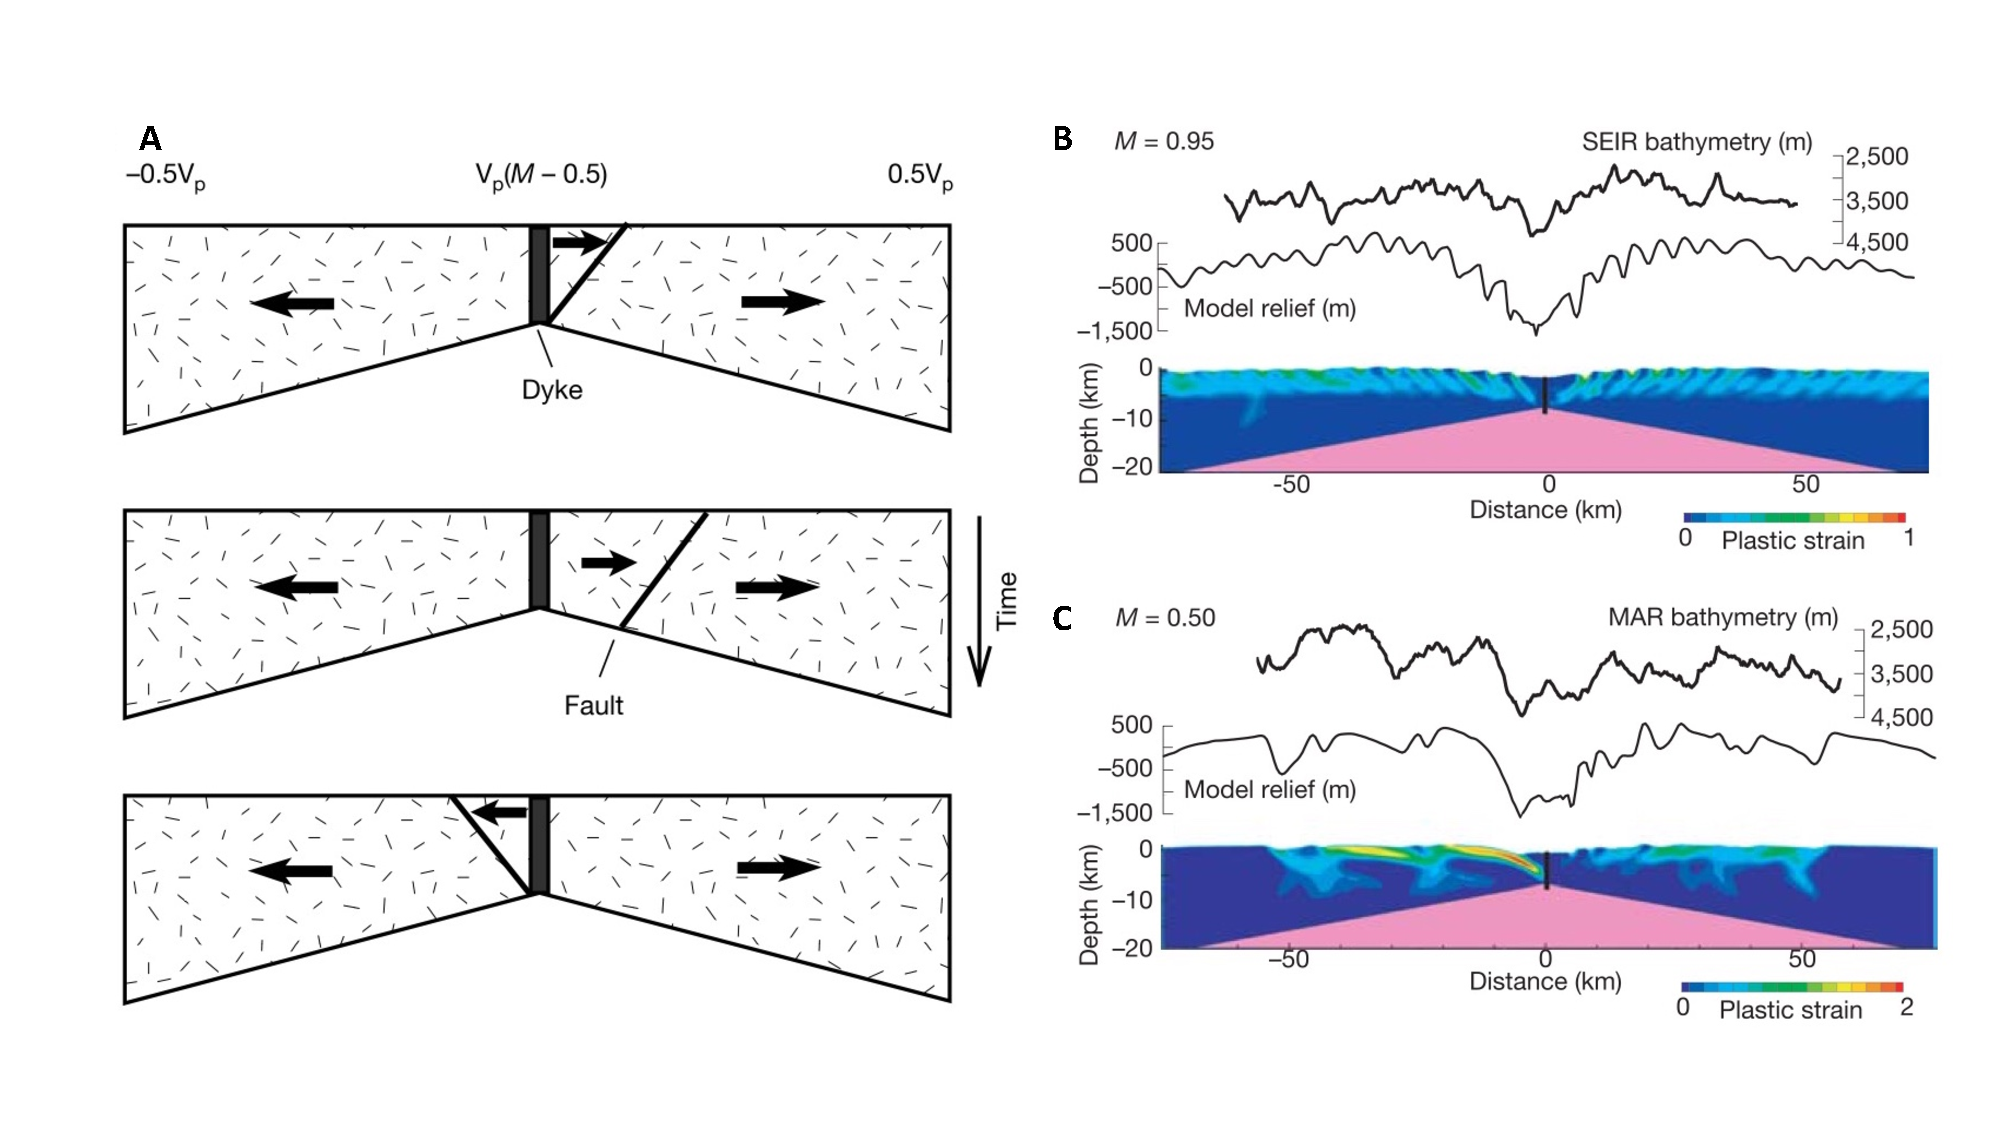
\includegraphics[width=0.99\linewidth]{./figs/fig1.pdf}
	\caption{\textbf{A.} Cartoon showing how the hanging-wall block of a fault may migrate during ridge stretching as a function of time for 0.5 $<$ M $<$ 1.0. \textbf{B.} Plastic strain distribution and surface relief from the numerical model with M = 0.95. High plastic strain represents shearing on faults and the bathymetric profile across the Southeast Indian Ridge (SEIR) is shown for comparison. \textbf{C.} Same as \textbf{B} but for M = 0.5. A bathymetric profile from the Mid-Atlantic Ridge (MAR) is shown for comparison. From \citet{Buck2005}}
	\label{fig:mfactor}
\end{figure}

%\section{Numerical approach}
%\note[EC]{Let's reorganize ``Numerical approach'' as follows: Governing equations, Numerical methods for approximate solution. Then, ``Model Setup'' becomes a new (sub-)section.}

\section{Governing equation}

\section{Numerical methods for approximate solution}
The FLAC (Fast Lagrangian Analysis of Continua) method \citep{Cundall1982, Poliakov1993} solves the equations describing conservation of momentum
\begin{align}
 \frac{D v_i}{D t} & = \frac{\partial \sigma_{ij}}{\partial x_{j}} + \rho g
\end{align}
\noindent and energy
\begin{align}
 \rho \bigg[ \frac{\partial u_i}{\partial t} + u_j\frac{\partial u_i}{\partial x_j} \bigg] & = -\frac{\partial P}{\partial x_{i}} + \rho g + \mu \frac{\partial^2 u_i}{\partial x_j \partial x_j}
\end{align}
\noindent for a visco-elastic-plastic continuum in 2-D Cartesian geometry \citep{Lavier2002}. By solving the conservation of momentum, the accelerations are integrated in time to give updated velocities, strains and strain rates. In addition, using the constitutive laws the strains and strain rates are used to calculate new elastic and viscous stresses. These stresses are used to determine the accelerations for the next step of calculation.


\section{Model Setup}
For visco-elastic deformation, the material behaves as a Maxwell solid. I follow the dry diabase power law rheology \citep{Kirby1987, Chen1990}. Plastic yielding is controlled by Mohr-coulomb theory, in which cohesion is a function of the total accumulated plastic strain \citep{Poliakov1998}. Cohesion decreases linearly from its initial value 44 MPa to the minimum value of 4 MPa.

\begin{figure}[!htb]
	\centering
	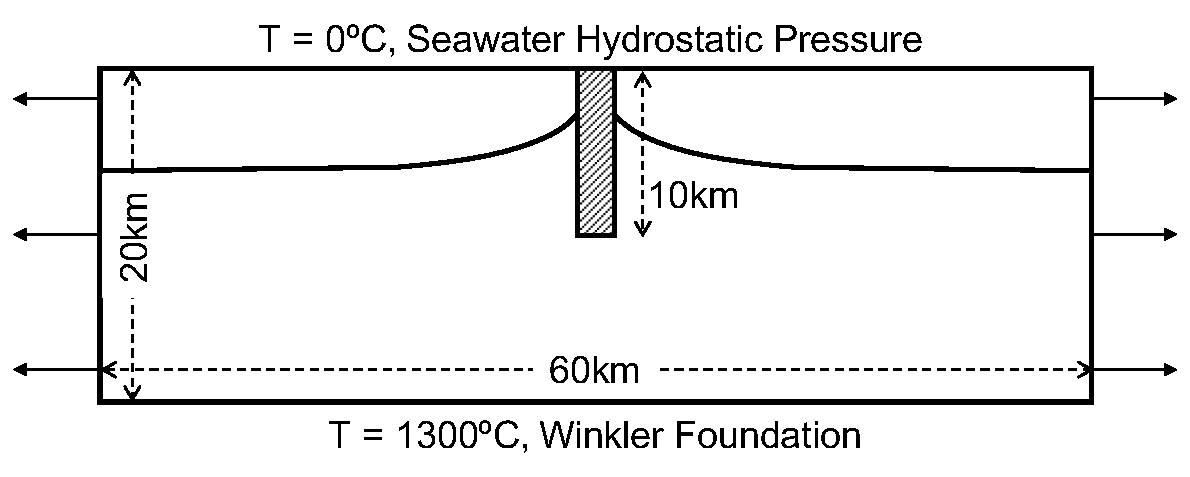
\includegraphics[width=0.8\linewidth]{./figs/modelsetup.pdf}
	\caption{ .}
	\label{fig:modelsetup}
\end{figure}

\begin{figure}[!htb]
	\centering
	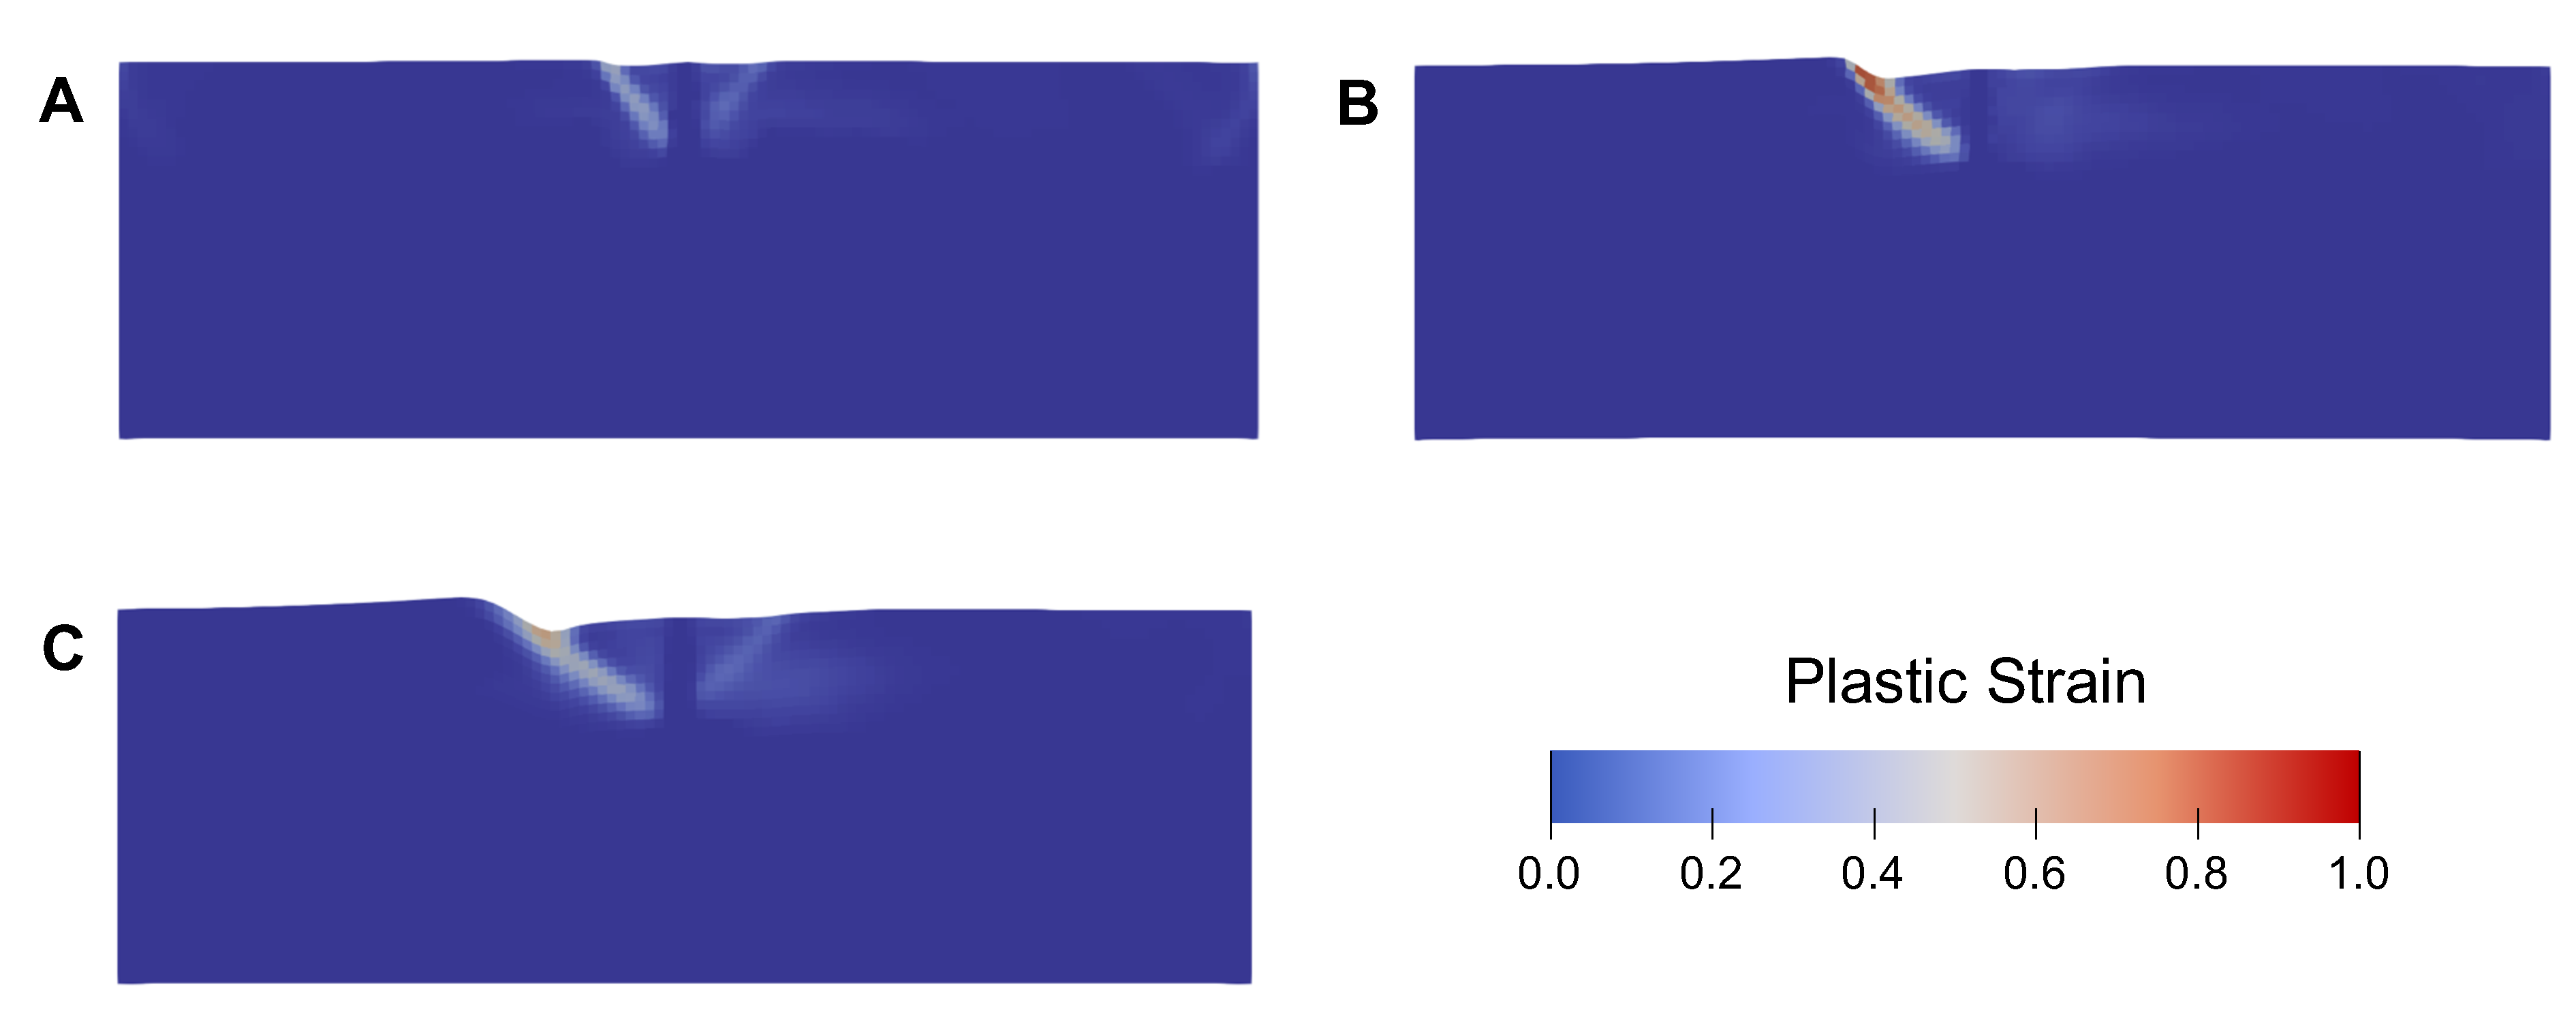
\includegraphics[width=0.9\linewidth]{./figs/fault_stage.pdf}
	\caption{ Snapshots of the kinematic model (M = 0.8) representing stages of the fault evolution. The fault evolution can be divided as three stages. \textbf{A.} Incipient stage: new fault occurs on left side of the ridge axis.  \textbf{B.} Mature stage: fault heave increases and fault dip decreases as fault grows. \textbf{C.} Terminal stage: fault becomes inactive and is replaced by a new-near axis fault on the other side of ridge axis.}
	\label{fig:faultstage}
\end{figure}

The model domain is rectangular with centered ridge axis. All models have 60 km wide and 20 km deep of domain sizes with the grid of 0.5 $\times$ 0.5 km. At the top boundary, I apply seawater hydrostatic pressure while at the bottom side isostatic equilibrium is realized by means of the Winkler foundation. I apply dynamic force boundary conditions at the lateral model sides, such that at the initial stage, the boundary force is linearly increasing, allowing the plate to reach the typical sea-floor spreading rates (2.5 cm/yr). This approach is feasible if the model shows brittle failure with constant boundary forces. Hereafter, boundary force for force boundary conditioned model is defined by averaging internal force of kinematic model from the mature stage of the fault (Figure \ref{fig:faultstage}B) to the moment of incipient stage of the fault (Figure \ref{fig:faultstage}A) on the other side of the ridge axis. I use residual force defined as a sum of constant boundary force and internal force (Equation \ref{Fres}).

\begin{figure}[!htb]
	\centering
	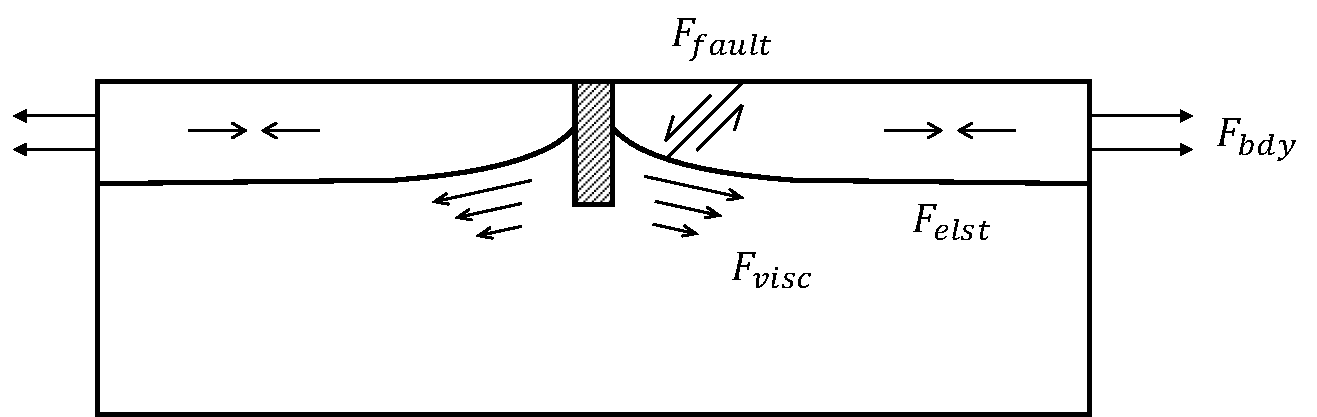
\includegraphics[width=0.9\linewidth]{./figs/force.pdf}
	\caption{ Schematic illustration of the internal forces and boundary forces applying to the model.}
	\label{fig:forcescheme}
\end{figure}
\begin{align} \label{Fres}
F_{res} & = F_{int} + F_{bdy} \\
 & = F_{fault} + F_{elst} + F_{visc} + F_{bdy}
\end{align}

\chapter{Results}

\section{Kinematic models}


\section{Force boundary models}

\subsection{F=0 models}

\subsection{Plate velocity varies with fault evolution}

Fault development at a ridge affects plate velocity. In kinematic models, normal fault migrates away from the axis at a rate $U = 2v(M-0.5)$, where $v$ is a constant plate driving velocity (Figure \ref{fig:hangingwall}) \citep{Buck2005}. Similarly, in the cases of force driven model, interaction between dynamic driving velocity from boundary force and opposite direction velocity from normal fault controls the plate speed in force. The plate containing active fault is slower than another plate.

%The plate velocity variation by fault evolution takes part in short term and small magnitude.

\begin{figure}[!htb]
	\centering
	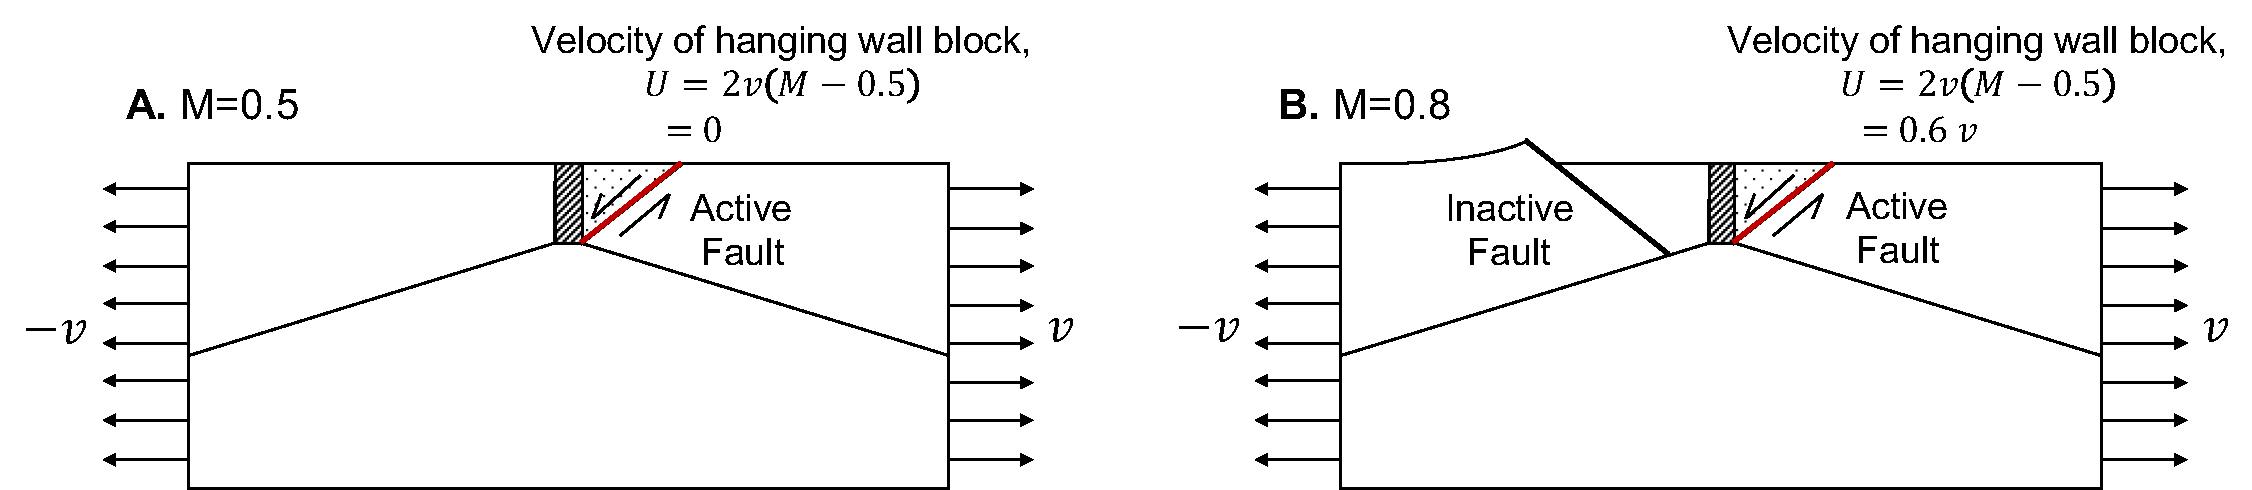
\includegraphics[width=0.99\linewidth]{./figs/hangingwall.pdf}
	\caption{\textbf{A.} Schematic model showing velocity of plate including active fault at mid-ocean ridges driven by velocity when M = 0.5. \textbf{B.} Same as \textbf{A} but for M = 0.8. }
	\label{fig:hangingwall}
\end{figure}

\subsubsection{M = 0.5}

When $M=0.5$, half portion of plate spreading is accommodated by faulting and the master detachment fault forms because the fault ceases to migrate.
In my model, the expected faulting mode lasts until 650 Kyrs.

%Unlike velocity-driven model, force-driven model shows significant velocity changes over time. The detachment fault forms at 50Kyrs on left side of the spreading axis. After *yrs, the left plate moves slowly.

\begin{figure}[!htb]
	\centering
	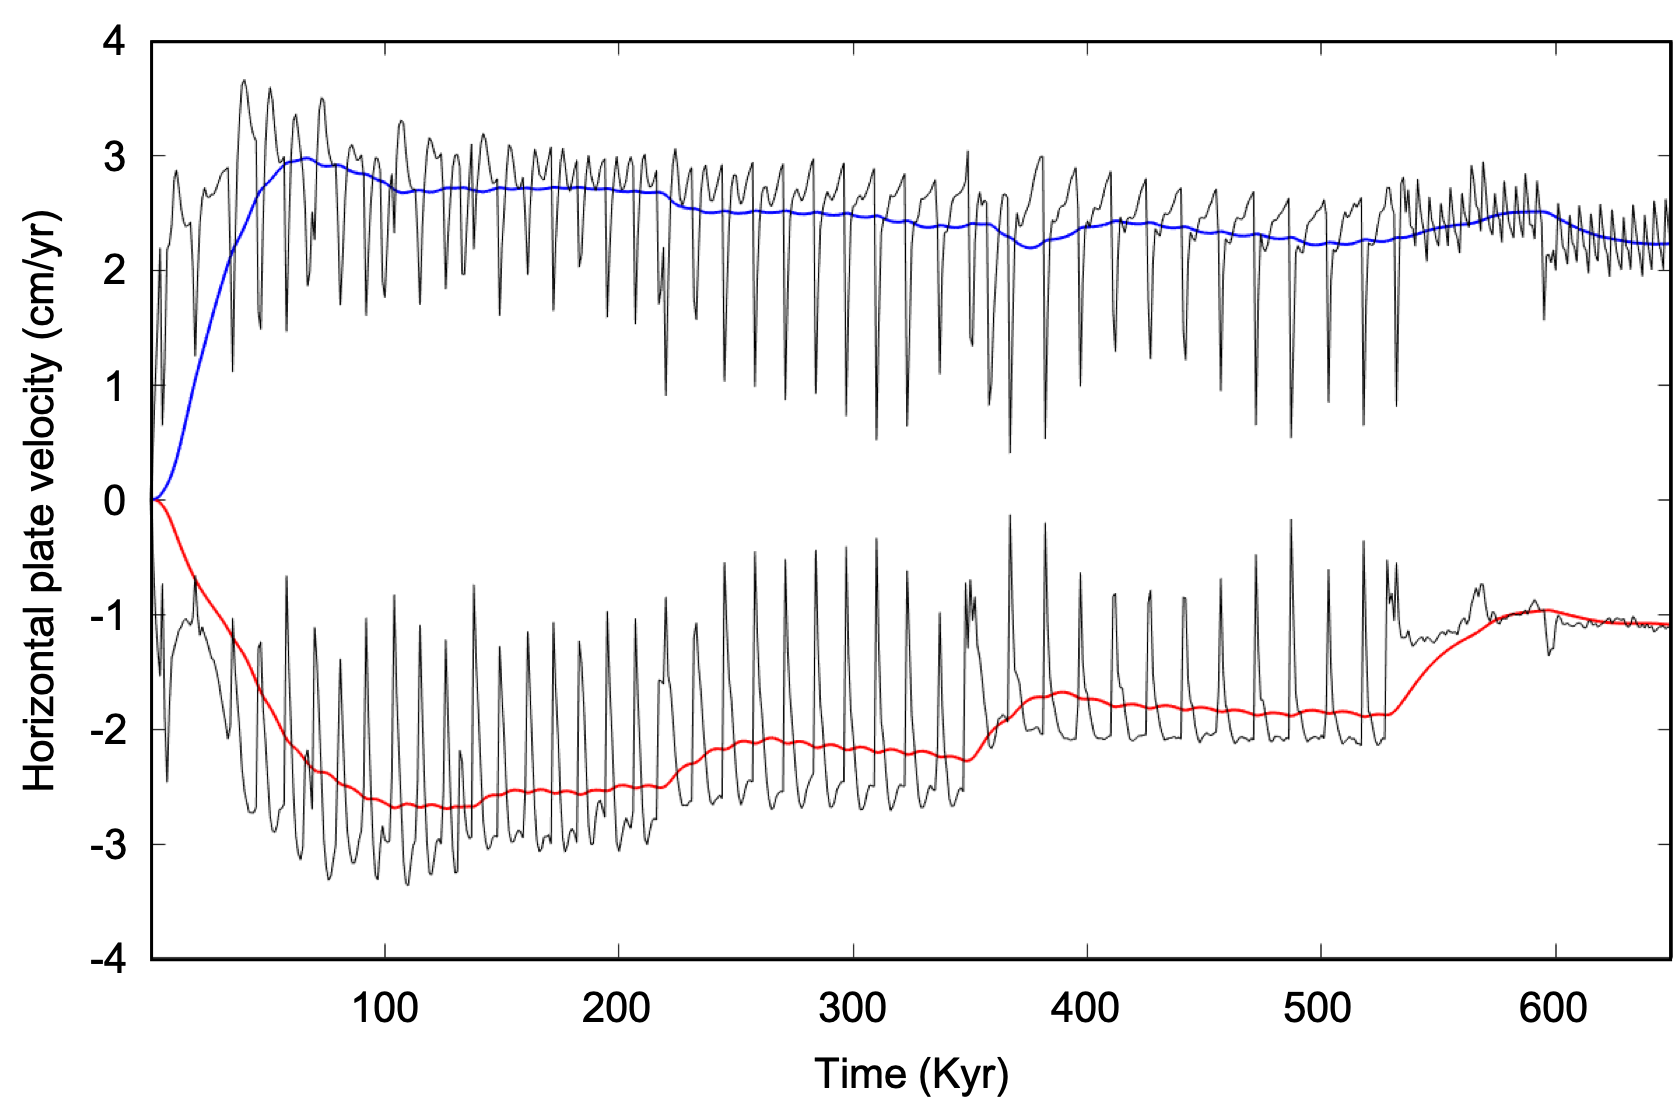
\includegraphics[width=0.99\linewidth]{./figs/m05vel.png}
	\caption{Plate velocity obtained from M = 0.5 model results. Abnormal peaks from remeshing effects are filtered out.}
	\label{fig:m05vel}
\end{figure}

\subsubsection{M = 0.8}

When $M=0.8$, fault migrates toward off-axis. The fault eventually becomes inactive and is replaced by new and near-axis fault.

\begin{figure}[!htb]
	\centering
	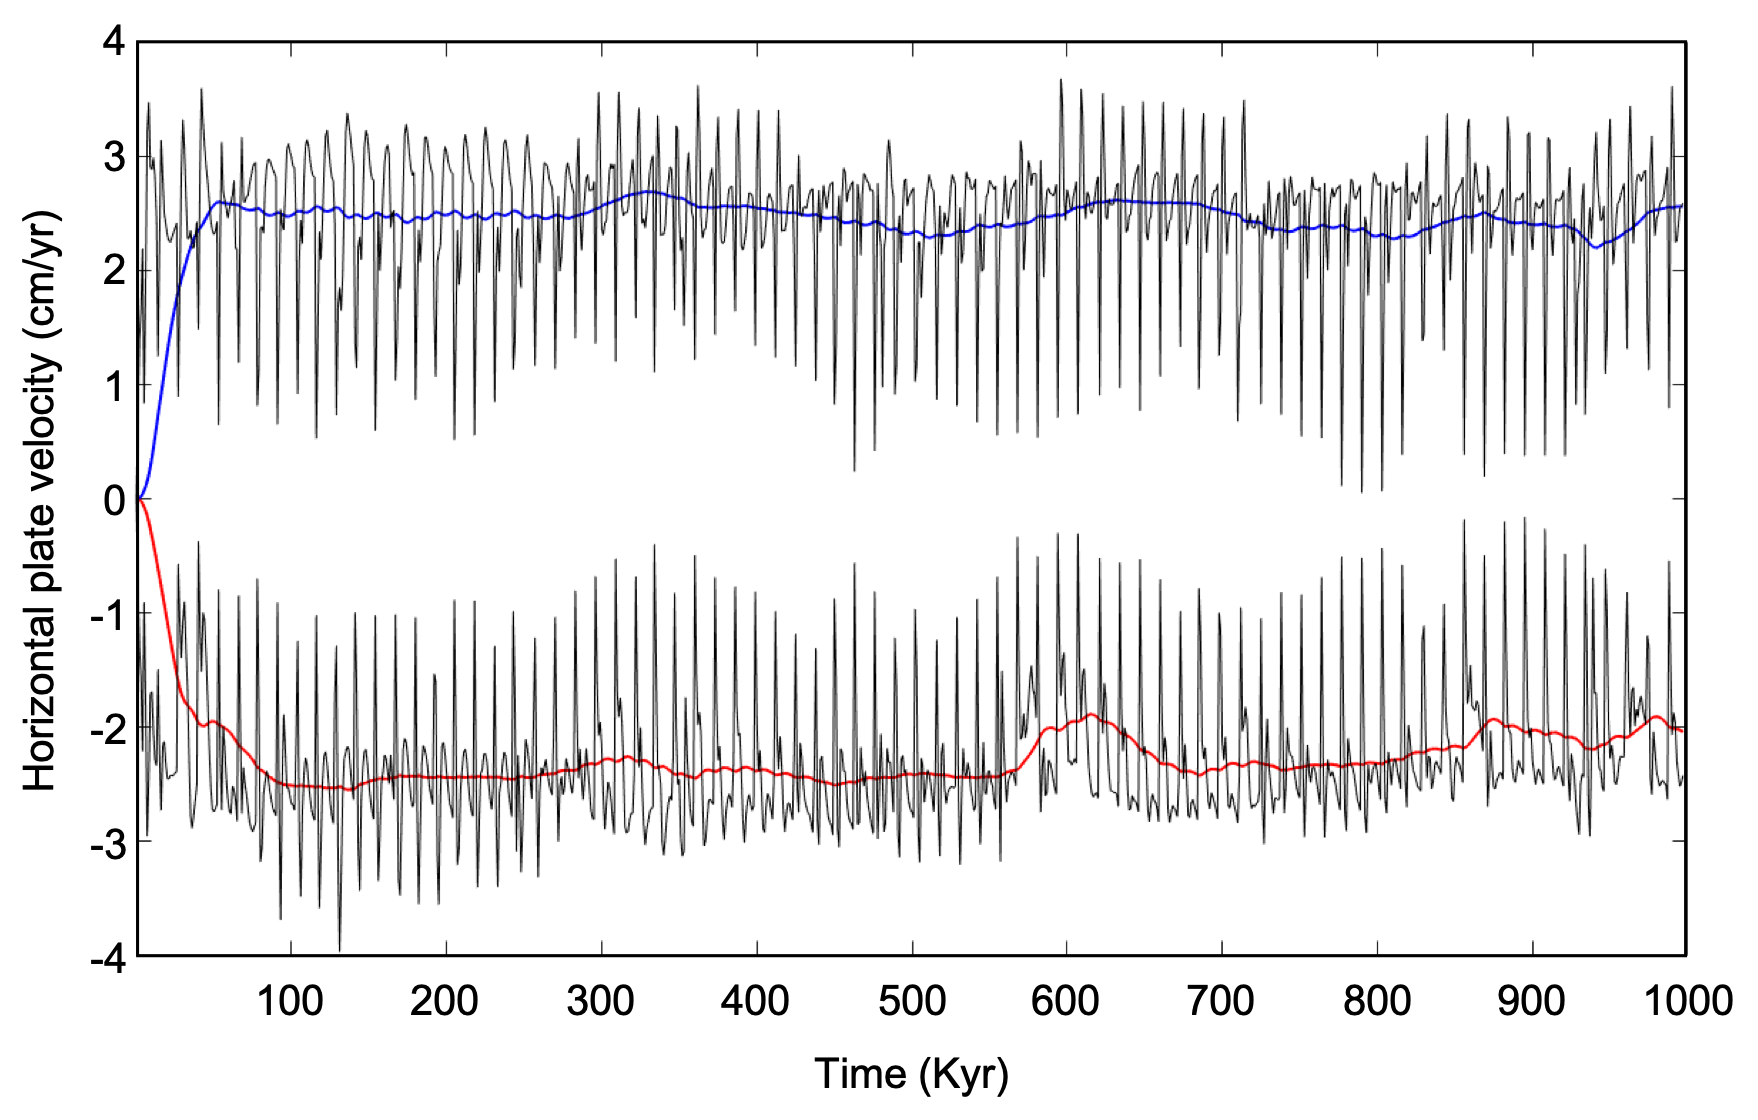
\includegraphics[width=0.99\linewidth]{./figs/m08vel.png}
	\caption{Plate velocity obtained from M = 0.8 model results. Abnormal peaks from remeshing effects are filtered out.}
	\label{fig:m08vel}
\end{figure}

%\begin{table}[h!]
%	\centering
%	\caption{1-D model used for routine earthquake locations and as the initial model for traditional 3-D tomographic images \citep{nakajima2001three}.}
%	\label{tab:vmodel}
%	\begin{tabular}{ccc}
%		\toprule
%		Depth, km & P Wave Velocity, km/s & S Wave Velocity, km/s\\
%		\midrule
%		0 & 5.60 & 3.24\\
%		10 & 6.00 & 3.46\\
%		25 & 6.79 & 3.92\\
%		40 & 7.72 & 4.34\\
%		65 & 7.79 & 4.38\\
%		90 & 7.92 & 4.45\\
%		120 & 8.01 & 4.50\\
%		150 & 8.09 & 4.55\\
%		\bottomrule
%	\end{tabular}
%\end{table}

\section{Thermal state}

Long term and large magnitude variation which cannot be explained by fault evolution may be caused by changes of the plate thermal state. By varying heat injection rate of the model, different behaviors of long term and large magnitude plate speed variation are observed. 

%\begin{table}[h!]
%	\centering
%	\caption{Percentage of P-wave and S-wave RMS reduction with respect to the original for different smoothing values after 20 iterations. The P-wave RMS reduction when using smoother = 10 is negative, which means that the inversion does not converge under this configuration.}
%	\label{tab:rms_reduction}
%	\begin{tabular}{ccc}
%		\toprule
%		Smoother & P-wave RMS reduction & S-wave RMS reduction \\
%		\midrule
%		10 & -14.7398\% & 9.9293\% \\
%		64 & 20.3963\% & 17.455\% \\
%		100 & 19.2424\% & 14.1327\% \\
%		128 & 17.3583\% & 7.5101\% \\
%		256 & 11.8203\% & 2.3572\% \\
%		\bottomrule
%	\end{tabular}
%\end{table}

\chapter{Discussion}

\chapter{Conclusion}

\bibliography{references}     % before changing bibliographystyle, remove *.bbl files in your working directory
\bibliographystyle{agsm.bst}  % the closest style to the University of Memphis Thesis Style Guide

\end{document}
